\documentclass[10pt]{article}

\usepackage{graphicx}
\usepackage{float}
\usepackage{comment}
\usepackage{wrapfig}
\usepackage{amsmath}
\usepackage{amssymb}
\usepackage{subfigure}
\usepackage{caption}
\usepackage{subcaption}
\usepackage{siunitx}
\usepackage{enumitem}
\usepackage{xcolor}
\usepackage{url}
\usepackage{fontspec}
\usepackage[backend=bibtex,bibstyle=numeric]{biblatex}
\usepackage{filecontents}
\addbibresource{references.bib}
\setmainfont{Latin Modern Roman}
%\bibliographystyle{amsplain}
%\bibliography{references}


\title{Studio dello stato attivo del blazar Mrk421 con ASTRI Mini-Array​}

\author{Giacomo Spaccini}
\date{17 Dicembre 2026}

\begin{document}


\maketitle

\section{Introduzione}

\newpage

\section{Very High Energy AstroPhysics}

L'astrofisica contemporanea si divide in molte branche, tutte connesse dallo studio di tutti quei messaggeri cosmici che consentono di osservare gli eventi e processi che caratterizzano l'Universo.
\\
Tra i vari approcci esistenti allo studio del cosmo, quello legato al lavoro mostrato in questa tesi è l'Astrofisica delle Altissime Energie (in inglese \textit{Very High Energy AstroPhysics} o, in breve, VHEAP), la quale si occupa prevalentemente dello studio dei fotoni gamma che appartengono, per l'appunto, alla fascia delle altissime energie, ovvero da circa $ 30 \hspace{3 pt} \unit{GeV}$ fino al centinaio di $ \unit{TeV} $ \cite{GRA2018}.
\\

\subsection{Introduzione all'astrofisica delle altissime energie}

I fotoni sono da sempre stati i messaggeri privilegiati nello studio dell'Universo, sin dagli albori dello studio del cielo attraverso la luce visibile sino ai giorni d'oggi, dove lo spettro studiato varia in energia dai $\unit{keV}$ dello studio della radioastronomia e radioastrofisica fino ai $\unit{PeV}$ tipici dell'astrofisica delle energie estreme.
\\
Uno spettro che varia per oltre 12 ordini di grandezza, ed ogni banda spettrale corrisponde a certi tipi di informazioni estraibili sull'Universo e differenti sistemi di rivelazione.

Il primo ambito è quello delle onde radio, con lunghezze d'onda che variano tra i $ 10^{-3} \hspace{3 pt} \unit{m} $ ed i $ 10^2 \hspace{3 pt} \unit{m} $, che consentono di studiare sia sorgenti interne al sistema solare, come Giove o lo stesso Sole, che sorgenti più lontane, come ad esempio quasar, pulsar o nuclei galattici attivi (in inglese \textit{Active Galactic Nuclei}, in breve AGN) fino a consentire di rilevare la radiazione cosmica di fondo, ovvero la radiazione residua attribuita al Big Bang, il cui picco è evidente nella figura \ref{GUPS}.


\begin{figure}[H]
	\centering
	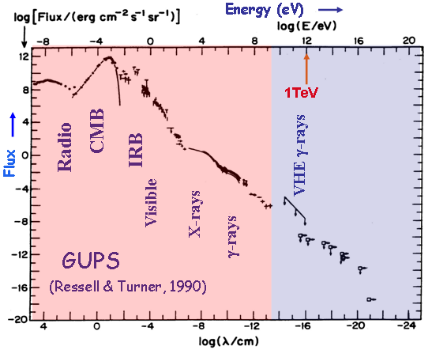
\includegraphics[width = 0.55\textwidth]{./Immagini/GreatPhotonSpectrum.png}
	\caption{Si può vede chiaramente il picco associato alla radiazione cosmica di fondo e si nota anche lo spettro  dei fotoni ad altissima energia. \cite{FRiA} }
	\label{GUPS}
\end{figure}


\begin{comment}
\vspace{10 pt}



\begin{wrapfigure}{1\textwidth} 
	%\vspace{-20pt}
	\begin{center}
		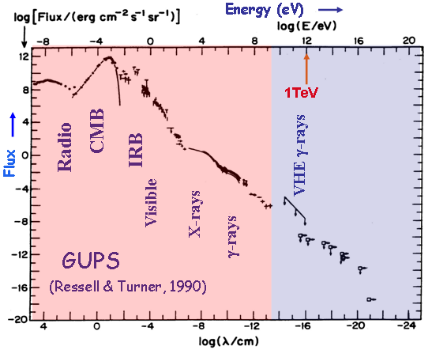
\includegraphics[width = 1\textwidth]{./Immagini/GreatPhotonSpectrum.png}
		
	\end{center}
	%\vspace{-20pt}
	\vspace{1pt}
\end{wrapfigure}

\vspace{10 pt}
\end{comment}

Si passa poi all'infrarosso, la banda spettrale tipica delle emissioni di corpi con temperature che arrivano fino alle migliaia di kelvin e la cui radiazione tende a superare ostacoli come le nubi di polvere interstellare e consente di studiare sorgenti che sarebbero oscurate in altre bande.
\\

Diminuendo ancora la lunghezza d'onda ed arrivando tra gli $800 \hspace{3 pt} \unit{nm}$ ed i $300 \hspace{3 pt} \unit{nm}$ circa si giunge allo spettro visibile, la banda spettrale più a lungo studiata e che è dominata dall'emissione di corpi con temperature più alte, che arrivano alle decine di migliaia di kelvin, come ad esempio le stelle.

Come per le onde radio, anche la radiazione visibile è tranquillamente studiabile da terra, dato che l'atmosfera è abbondantemente trasparente a queste frequenze.
\\

Aumentando ulteriormente l'energia della radiazione osservata si incontrano le emissioni che ricadono nell'ultravioletto e, soprattutto, nei raggi X, radiazioni emesse prevalentemente da fenomeni molto intensi e corpi dalle temperature che superano i milioni di kelvin.

Nonostante la difficoltà nell'osservare questi fotoni per via dell'opacità dell'atmosfera, il che spesso richiede di avere rilevatori in orbita oltre l'atmosfera o persino sonde spaziali, lo studio dei raggi X di origine extraterrestre ha consentito di analizzare processi non percepibili nell'ottico e popolando il cielo di tantissime sorgenti altrimenti invisibili.
\\

Infine si raggiunge lo spettro dei fotoni gamma, i fotoni più energetici, che aprono una finestra sugli eventi più estremi ed interessanti dell'Universo, ma prima di parlarne è necessario definire cosa emetta radiazioni elettromagnetiche.
\subsection{Processi di produzione dei fotoni gamma}
La radiazione elettromagnetica nell'Universo viene emessa sostanzialmente attraverso due processi, che vengono definiti come "emissione termica" e "emissione non termica".
\\
L'insieme degli eventi caratterizzati da un'emissione termica, detto "Universo termico", è costituito da tutti quei corpi in equilibrio termodinamico e che, conseguentemente, hanno uno spettro di radiazione che segue quello del corpo nero.
Dunque, lo spettro di emissione dell'Universo termico segue la legge di Wien, la legge che enuncia l'inversa proporzionalità tra la lunghezza d'onda del picco di emissione e la temperatura del corpo. Per questo, l'Universo termico ha un'impronta prevalentemente presente dall'infrarosso fino ai raggi X.
\\

l'Universo non-termico, invece, è composto da tutti gli eventi astrofisici che non avvengono all'equilibrio termodinamico ed emette soprattutto nello spettro delle onde radio e dei raggi gamma. Questo genere di emissione, in particolare quella nello spettro dei fotoni gamma, è il risultato di particelle ultrarelativistiche accelerate dalla trasformazione di energia gravitazionale in energia elettromagnetica \cite{VHEGA}.
\\

Nello specifico, la gran parte di questi fotoni sono emessi da elettroni, spesso in prossimità di eventi estremi come dischi di accrescimento o getti di plasma. Questi elettroni emettono per \textit{bremsstrahlung} (il cui spettro caratteristico è proporzionale all'inverso dell'energia emessa) o emettono radiazione si sincrotrone per via dei forti campi magnetici in cui sono immersi (il cui spettro caratteristico per elettroni ultra-relativistici è una \textit{power-law}).
\\
In particolare, avviene quello che viene definito \textit{self-synchrotron Compton}, o in breve SSC, ovvero il processo in cui un fotone emesso per radiazione di sincrotrone da un elettrone ultra-relativistico (tipicamente con un'energia tra quella dell'infrarosso e dei raggi X) interagisce per scattering Compton inverso con la popolazione di elettroni che l'ha emesso, ricevendo un aumento di energia anche di 10 ordini di grandezza.
\\
La distribuzione dei fotoni che interagiscono per scattering Compton inverso ha un picco nell'ordine di grandezza tra i $ \unit{GeV} $ ed i $ \unit{TeV} $, restituendo lo spettro tipico delle sorgenti di fotoni ad altissima energia, come la Crab Nebula.
\\
Un caso particolare di emissione dovuta allo scattering Compton inverso è quando, invece che interagire con la stessa popolazione elettronica che li ha emessi, i fotoni interagiscono con una seconda popolazione elettronica generata da cascate che trovano la loro origine in nuclei o protoni fortemente accelerati dai \textit{jet} \cite{grBLLAC}.
In questi casi, per via dell'origine dei fotoni dal decadimento secondario di mesoni, non solo l'energia è di un paio di ordini di grandezza maggiore rispetto alla controparte di SSC, ma proprio perchè sono fotoni emessi da cascate adroniche questi raggi gamma possono essere studiati per ottenere una maggior comprensione di come vengono prodotti i raggi cosmici \cite{VHEGA}.
\\
In questo ambito, il caso degli AGN è di particolare rilievo. Infatti, spesso i fotoni emessi come sopra descritto andrebbero facilmente incotro a collisioni con altri fotoni, più abbondati, nelle fasce energetiche inferiori e verrebbero assorbiti in un processo di produzione di coppia, ma poichè in questi corpi astrofisici la gran parte della materia che vi cade viene trasformata in \textit{jet} collimati e dalla direzione perpendicolare al disco di accrescimento, molti di questi fotoni gamma incontrano una particolarmente bassa popolazione di altri fotoni e dunque sfuggono all'assorbimento.
\\

In ultimo luogo, un ulteriore processo di produzione dei fotoni gamma viene considerato legato allo studio della materia oscura \cite{GRA2018}.

Infatti, in quello che viene definito \textit{top-down scenario}, si considera la possibilità che il decadimento o l'annichilimento di particelle esotiche, in particolare le WIMP (\textit{Weak Interactive Massive Particles}) possa produrre radiazione gamma.

In particolare, il flusso di questi fotoni gamma sarebbe direttamente proporzionale al tasso di annichilimento delle particelle considerate ed allo spettro che i singoli eventi di annichilimento produrrebbero.
Tuttavia, c'è da considerare che poichè le WIMP sono elettricamente neutre, questi processi sono alquanto rari e spesso dominati in flusso da quelli descritti in precedenza.

\newpage

\section{Telescopi Cherenkov ed ASTRI}

\newpage

\section{Panoramica di Markarian421}

\newpage

\section{Analisi}

\newpage

\section{Conclusioni}

\newpage

\section{Bibliografia}
\printbibliography

\end{document}
